
\section{Vecteurs de l'espace}
\activity{Vecteurs de l'espace}{6}{
Coffi et ses camarades se souviennent des notions de
vecteurs dans le plan. Puis ils s’interrogent sur ce
qu’il en est dans l’espace.
}
\subsection{Caractéristiques d'un vecteur de l'espace}
\consigne{Découverte}{6.1}{
\begin{minipage}{13cm}
	On considère le vecteur $\V{IJ}$ du dessin de l'armoire.
	\be \item Recopie et complète.
	%\begin{itemize}
	\par $\bullet$ Dans le plan $(ABC)$, on a : $\V{IJ}\text{\dots}\V{DC}$, car $IJCD$ est un parallélogramme.
	\par $\bullet$ Dans le plan $(LKJ)$, on a : $\V{IJ}\text{\dots}\V{LK}$, car $IJKL$ est un parallélogramme.
%	\end{itemize}
\vspace*{-0.3cm}
\info{Ainsi $\V{IJ}$ a un représentant dans le plan $(ABC)$ et aussi dans le plan $(LKJ)$, qui sont deux plans distinct. On dit que le vecteur $\V{IJ}$ est un vecteur de l'espace. L'ensemble des vecteurs de l'espace est noté $\mathcal{W}$}
\vspace*{-0.5cm}
\item \be \item Détermine les caractéristiques du vecteurs $\V{IJ}$.
\item Détermine les caractéristiques d'un vecteur quelconque de l'espace. (Tu distingueras le cas où le vecteur est nul et non nul).\ee\ee
\end{minipage}
\begin{minipage}{5cm}
\begin{tikzpicture}[scale=0.7]
\tkzInit[xmin=0,ymin=0,xmax=6,ymax=10]
%\tkzAxeXY
%\tkzGrid
\tkzDefPoints{0/0/E,4/0/A,4/3/I,0/3/L,4/7/D,0/7/H,5/1/B,1/1/F,5/4/J,1/4/K,5/8/C,1/8/G}
\tkzDefMidPoint(L,I)\tkzGetPoint{M}\tkzDefMidPoint(K,J)\tkzGetPoint{N}\tkzDefMidPoint(G,C)\tkzGetPoint{O}\tkzDefMidPoint(H,D)\tkzGetPoint{P}
\tkzDrawSegments(L,E E,A A,I I,L I,D D,H H,L D,C C,G G,H A,B B,J J,I J,C O,P)
\tkzDrawSegments[dashed](E,F F,B F,G L,K K,J P,M M,N N,O)
\tkzLabelPoints(A,B,F,M,I,J,K)
\tkzLabelPoints[left](E,L)\tkzLabelPoints[above](H,P,D,C,O,G)
\tkzLabelPoints[above right](N)
\end{tikzpicture}
\end{minipage}
}
\resultat{(à faire)}
\begin{definition}[s]
\par\ding{43} À deux points distincts $A$ et $B$ de l'espace, on peut associer deux vecteurs, le vecteur $\V{AB}$ et le vecteur $\V{BA}$.
\par \ding{43} Le point $A$ est appelé \textbf{origine} du vecteur $\V{AB}$ et le point $B$, son \textbf{extrémité}.
\par \ding{43} Le vecteur $\V{AB}$ est caractérisé par :
\begin{itemize}
	\item sa direction qui est celle de la droite $(AB)$.
	\item son sens qui est le sens de $A$ vers $B$.
	\item sa longueur ou sa norme qui est la distance $AB$.
\end{itemize}
\par \ding{43} Le vecteur $\V{AA}$ est le vecteur nul, noté $\V{0}$. Il n'a ni direction, ni sens, mais sa norme est $0$.
\par \ding{43} Dire que les vecteurs $\V{AB}$ et $\V{CD}$ sont égaux signifie :
\begin{itemize}
	\item qu'ils ont même direction ;
	\item qu'ils ont même sens ;
	\item qu'ils ont même norme.
\end{itemize}
\par \ding{43} Dire que les vecteurs $\V{AB}$ et $\V{CD}$ sont opposés signifie :
\begin{itemize}
	\item qu'ils ont même direction ;
	\item qu'ils sont de sens contraire ;
	\item qu'ils ont même norme.
\end{itemize}
%\par \ding{43} Si les points $A$, $B$, $C$ et $D$ étant quatre points non alignés de l'espace,  dire que $\V{AB}$ et $\V{CD}$ sont égaux signifie que le quadrilatère $ABCD$ est un parallélogramme.
%\par \ding{43} Dire que les vecteurs $\V{AB}$ et $\V{CD}$ sont colinéaires signifie qu'ils ont la même direction.
\end{definition}\\
\begin{propriete}[s]
\par \ding{43} Pour tout point $A$ et pour tout vecteur $\V{u}$ de l'espace, il existe un unique point $M$ de l'espace tel que $\V{AM}=\V{u}$\\
\hspace*{3cm} \begin{tikzpicture}[scale=0.8,vect/.style={->,shorten >=1pt,>=latex'}]
\tkzInit[xmin=0,ymin=0,xmax=8,ymax=8]
%\tkzAxeXY\tkzGrid
\tkzDefPoints{0/0/O,2/3/O',2/1/A}
\tkzDefParallelogram(O',O,A)\tkzGetPoint{M}
\tkzDrawPoints(A,M)
\tkzDrawSegments[vect](O,O' A,M)
\tkzLabelSegment(O,O'){$\V{u}$}
\tkzLabelPoints(A,M)
\end{tikzpicture}
\par \ding{43} Pour tout point $A$, $B$ et $C$ de l'espace on a : $\V{AB}+\V{BC}=\V{AC}$ (Relation de Chasles).
\par \ding{43} Pour tout points $A$, $B$, $C$ et $D$ non alignés de l'espace, on a :
\par \hspace*{2cm}$ABDC$ est un parallélogramme $\iff$ \begin{tabular}{||l}
$\V{AB}=\V{CD}$ ;\\
$\V{AC}=\V{BD}$ ;\\
$[AD]$ et $[BC]$ ont même milieu.
\end{tabular}
\par \hspace*{5cm} \begin{tikzpicture}[scale=0.8,vect/.style={->,shorten >=1pt,>=latex'}]
\tkzInit[xmin=0,ymin=0,xmax=8,ymax=8]
%\tkzAxeXY\tkzGrid
\tkzDefPoints{2/0/C,7/0/D,0/2/A,5/2/B}
\tkzDefMidPoint(B,C)\tkzGetPoint{I}
\tkzDrawPoint(I)
%\tkzLabelPoints[right=3pt](B,C)
\tkzDrawSegments[vect](A,B C,D)
\tkzDrawSegments[vect,color=blue](A,C B,D)
\tkzDrawSegments[dashed](A,D B,C)
\tkzMarkSegments[mark=|](A,I I,D)
\tkzMarkSegments[mark=||](C,I I,B)
\tkzLabelPoints[below](C,D)
\tkzLabelPoints[above](A,B,I)
\end{tikzpicture}
\end{propriete}
\subsection{Opérations sur les vecteurs}
\consigne{Opérations sur les vecteurs}{6.2}{
	On définit la somme de deux vecteurs de $\mathcal{W}$ ainsi que le produit d’un vecteur par un nombre réel de la même manière que dans le plan.
	\par Reprends le dessin ci-dessous, puis construits les vecteurs suivants : $\V{U}=\vec{v}+\vec{w}$ et $\V{V}=2\vec{u}-\vec{v}$
	\par \hspace*{3cm} \begin{tikzpicture}[scale=0.8,vect/.style={->,shorten >=1pt,>=latex'}]
	\tkzInit[xmin=0,ymin=0,xmax=6,ymax=6]
	%\tkzAxeXY\tkzGrid
	\tkzDefPoints{0/0/A,3/2/B,1/4/D,6/2/E}
	\tkzDrawSegments[vect](B,A B,D B,E)
	\tkzLabelSegment[below](B,A){$\V{u}$}
	\tkzLabelSegment[below](B,E){$\V{v}$}
	\tkzLabelSegment[above](B,D){$\V{w}$}
	\end{tikzpicture}
}
\resultat{(à faire)}
\begin{definition}[s]
Soit $\vec{u}$ et $\vec{v}$, deux vecteurs de $\mathcal{W}$. $A$, $B$ et $C$ des points de l'espace tels que : $\vec{u}=\V{AB}$ et $\vec{v}=\V{AC}$.
\par \ding{43} On appelle \textbf{somme des vecteurs $\vec{u}$ et $\vec{v}$}, le vecteur $\V{w}$ tel que $\V{w}=\vec{u}+\vec{v}$.
\par \hspace*{3cm}  \begin{tikzpicture}[scale=0.8,vect/.style={->,shorten >=1pt,>=latex'}]
\tkzInit[xmin=0,ymin=0,xmax=8,ymax=3]
%\tkzAxeXY\tkzGrid
\tkzDefPoints{2/0/C,7/0/D,0/2/A,5/2/B}
\tkzDrawSegments[vect,color=blue](A,C A,B)
\tkzDrawSegment[vect,color=red](A,D)
\tkzDrawSegments[dashed](B,D C,D)
\tkzLabelPoints[below](C)
\tkzLabelPoints[above](A,B)
\tkzLabelSegment(A,B){$\vec{u}$}
\tkzLabelSegment[left=3pt](A,C){$\vec{v}$}
\tkzLabelSegment[below](A,D){$\V{w}$}
\end{tikzpicture}
\par \ding{43} On appelle \textbf{multiplication du vecteur $\vec{u}$ par un nombre réel $\alpha$}, le vecteur noté $\alpha\vec{u}$ tel que :
\begin{itemize}
	\item $\alpha\vec{u}$ a la même direction que $\vec{u}$, si $\alpha\neq 0$.
	\item $\alpha\vec{u}$ a même sens que $\vec{u}$, si $\alpha >0$.
	\item $\alpha\vec{u}$ a un sens contraire à celui de $\vec{u}$, si $\alpha <0$.
	\item la norme de $\alpha \vec{u}$, notée $\left\|\alpha\vec{u}\right\|=\lvert\alpha\rvert\times \left\|\vec{u}\right\|$.
\end{itemize}
\end{definition}\\
\begin{propriete}[s]
Pour tous vecteurs $\vec{u}$, $\vec{v}$ et $\V{w}$, pour tous nombres réels $\alpha$ et $\beta$, on a :
\par \begin{minipage}{0.5\linewidth}
	\par $\blacktriangleright$ $\big(\alpha \vec{u}=\vec{0}\big)\iff \big(\alpha=0\text{ ou }\vec{u}=\vec{0}\big)$\\
	 \par$\blacktriangleright$ $\alpha\textbullet\big(\beta\vec{v}\big)=\big(\alpha.\beta\big)\textbullet\vec{u}=\beta\textbullet\big(\alpha\textbullet\vec{u}\big)$\\
	\par $\blacktriangleright$ $\big(\alpha+\beta\big).\vec{u}=\alpha\vec{u}+\beta\vec{u}$\\
	\par $\blacktriangleright$ $\alpha\big(\vec{u}+\vec{v}\big)=\alpha\vec{u}+\alpha\vec{v}$\\
	\par $\blacktriangleright$ $1.\vec{u}=\vec{u}$
\end{minipage}
\end{propriete}
\subsection{Vecteurs colinéaires}
\begin{definition}
Deux vecteurs $\vec{u}$ et $\vec{v}$ de $\mathcal{W}$ sont dits \textbf{colinéaires}, lorsque l'un d'eux est le vecteur nul ou bien lorsque les deux vecteurs ont la même direction, c'est-à-dire, s'il existe un nombre réel $\alpha$ tel que $\vec{u}=\alpha\vec{v}$ ou $\vec{v}=\alpha \vec{u}$. 
\end{definition}
\subsection{Combinaisons linéaires}
\consigne{Combinaisons linéaires}{6.3}{
	\vspace*{-0.8cm}
\begin{minipage}{12.5cm}
En considérant le dessin de l'armoire ci-contre :
\be \item Construis sur la figure le vecteur $\vec{u}=\V{LK}+2\V{GO}+\F{1}{2}\V{LH}$.
\item On désigne par $Q$, le milieu de $[IA]$.
\be \item Les vecteurs $\V{QM}$ et $\V{LA}$ sont-ils colinéaires ? Justifie ta réponse.
\item Cite deux vecteurs non colinéaires.\ee
\item \be \item Exprime le vecteur $\V{MP}$ en fonction de $\V{HM}$ et $\V{MD}$.
\item Que représente le vecteur $\V{MP}$ pour les vecteurs $\V{HM}$ et $\V{MD}$ ?\ee\ee
\end{minipage}
%\vspace*{0.5cm}
\begin{minipage}{5cm}
	\begin{tikzpicture}[scale=0.7]
	\tkzInit[xmin=0,ymin=0,xmax=6,ymax=10]
	%\tkzAxeXY
	%\tkzGrid
	\tkzDefPoints{0/0/E,4/0/A,4/3/I,0/3/L,4/7/D,0/7/H,5/1/B,1/1/F,5/4/J,1/4/K,5/8/C,1/8/G}
	\tkzDefMidPoint(L,I)\tkzGetPoint{M}\tkzDefMidPoint(K,J)\tkzGetPoint{N}\tkzDefMidPoint(G,C)\tkzGetPoint{O}\tkzDefMidPoint(H,D)\tkzGetPoint{P}
	\tkzDrawSegments(L,E E,A A,I I,L I,D D,H H,L D,C C,G G,H A,B B,J J,I J,C O,P)
	\tkzDrawSegments[dashed](E,F F,B F,G L,K K,J P,M M,N N,O)
	\tkzLabelPoints(A,B,F,M,I,J,K)
	\tkzLabelPoints[left](E,L)\tkzLabelPoints[above](H,P,D,C,O,G)
	\tkzLabelPoints[above right](N)
	\end{tikzpicture}
\end{minipage}
}
\resultat{(à faire)}
\begin{definition}
\begin{minipage}{10cm}
	Soit $\vec{u}$ et $\vec{v}$ des vecteurs de $\mathcal{W}$. Tout vecteur de la forme $\alpha\vec{u}+\beta\vec{v}$, où $\alpha$ et $\beta$ sont des nombres réels, est appelé \textbf{combinaison linéaire} des vecteurs $\vec{u}$ et $\vec{v}$. $\alpha$ et $\beta$ sont les coefficients respectifs de $\vec{u}$ et $\vec{v}$.
\end{minipage}\hspace*{0.5cm}
\begin{minipage}{7cm}
\begin{tikzpicture}[scale=0.8,vect/.style={->,shorten >=1pt,>=latex'}]
\tkzInit[xmin=0,ymin=0,xmax=6,ymax=6]
%\tkzAxeXY\tkzGrid
\tkzDefPoints{0/0/A,4/0/B,2/2/D}
\tkzDefParallelogram(D,A,B)\tkzGetPoint{C}
\tkzDefPoints{1/1/A',1.5/0/B'}
\tkzDrawSegments[vect](A,A' A,C A,B' A,B A,D)
\tkzDrawSegment[vect,color=blue](A,C)
\tkzLabelSegment[below](A,B'){$\V{u}$}
\tkzLabelSegment[below](B',B){$\alpha\V{u}$}
\tkzLabelSegment[left](A,A'){$\V{v}$}
\tkzLabelSegment[left](A',D){$\beta\V{v}$}
\tkzLabelSegment[pos=0.6,above=2pt](A,C){$\alpha\V{u}+\beta\V{v}$}
\tkzDrawSegments[color=red,dashed](B,C C,D)
%\tkzDrawPolygon(A,B,C,D)
\end{tikzpicture}
\end{minipage}
\end{definition}\\\\
 \begin{propriete}
	$\vec{u}$ et $\vec{v}$ sont colinéaires si et seulement si il existe une combinaison linéaire de ces vecteurs qui soit nulle sans que ces coefficients soient tous les deux nuls, c'est-à-dire :
	\par $\vec{u}$ et $\vec{v}$ sont colinéaires si et seulement s'il existe un couple $\coord{\lambda}{\mu}\neq \coord{0}{0}$ tel que : $\lambda\vec{u}+\mu\vec{v}=\vec{0}$.
	\end{propriete}
\subsection{Vecteurs coplanaires}
\begin{definition}
Trois vecteurs $\vec{u}$, $\vec{v}$ et $\V{w}$ de $\mathcal{W}$ tels que $\vec{u}=\V{AB}$, $\vec{v}=\V{AC}$ et $\V{w}=\V{AD}$ sont dits \textbf{coplanaires} si et seulement si les points $A$, $B$, $C$ et $D$ sont dans un même plan.
\end{definition}
\begin{remark}
\ding{43} Deux vecteurs $\vec{u}$ et $\vec{v}$ sont toujours coplanaires.
\par \ding{43} Trois vecteurs $\V{OA}$, $\V{OB}$ et $\V{OC}$ sont non coplanaires si et seulement si les points $O$, $A$, $B$ et $C$ sont les sommets d'un tétraèdre.
\par \ding{43} Si $\vec{u}$ et $\vec{v}$ sont colinéaires, alors, pour tout vecteur $\V{w}$, les trois vecteurs $\vec{u}$, $\vec{v}$ et $\V{w}$ sont coplanaires.
\end{remark}
\begin{propriete}
		 Soit $\vec{u}$, $\vec{v}$ et $\V{w}$, trois vecteurs de $\mathcal{W}$ tels que $\vec{u}$ et $\vec{v}$ sont non colinéaires.
		\par $\vec{u}$, $\vec{v}$ et $\V{w}$ sont coplanaires si et seulement si $\V{w}$ est une combinaison linéaire de $\vec{u}$ et $\vec{v}$.
\end{propriete}
\consigne{Approfondissement}{6.4}{
	On considère le compartiment $ABFEIJKL$ de l'armoire.
	\be \item Les vecteurs $\V{AB}$, $\V{BF}$ et $\V{KJ}$ sont-ils coplanaires ?
	\item Démontre que les vecteurs $\V{AB}$, $\V{AE}$ et $\V{AI}$ sont non coplanaires.\ee
}\resultat{(à faire)}
\consigne{Propriétés relatives aux vecteurs coplanaires}{6.5}{
	\begin{minipage}{13cm}
\be \item Dans chacun des cas suivants, dis si les vecteurs sont coplanaires ou non.
\begin{itemize} 
\item $\V{AE}$, $\V{AD}$ et $\V{AM}$.
\item $\V{DC}$, $\V{ON}$ et $\V{HP}$.
\item $\V{LK}$, $\V{MN}$ et $\V{DJ}$
\item $\V{AP}$, $\V{KM}$ et $\V{GP}$
\end{itemize}
\item soit $\vec{u}$, $\vec{v}$ et $\V{w}$ trois vecteurs de $\mathcal{W}$.
\be \item Démontre que s'il existe des nombres réels $\alpha$, $\beta$ et $\gamma$ tels que 
\par $\alpha\vec{u}+\beta\vec{v}+\gamma\V{w}=\vec{0}$, alors $\vec{u}$, $\vec{v}$ et $\V{w}$ sont coplanaires.
\item Démontre que si $\vec{u}$, $\vec{v}$ et $\V{w}$ sont coplanaires, alors il existe des nombres réels $\alpha$, $\beta$ et $\gamma$ non tous nuls tels que $\alpha\vec{u}+\beta\vec{v}+\gamma\V{w}=\vec{0}$.\ee\ee
	\end{minipage}
	\begin{minipage}{5cm}
		\begin{tikzpicture}[scale=0.7]
		\tkzInit[xmin=0,ymin=0,xmax=6,ymax=10]
		%\tkzAxeXY
		%\tkzGrid
		\tkzDefPoints{0/0/E,4/0/A,4/3/I,0/3/L,4/7/D,0/7/H,5/1/B,1/1/F,5/4/J,1/4/K,5/8/C,1/8/G}
		\tkzDefMidPoint(L,I)\tkzGetPoint{M}\tkzDefMidPoint(K,J)\tkzGetPoint{N}\tkzDefMidPoint(G,C)\tkzGetPoint{O}\tkzDefMidPoint(H,D)\tkzGetPoint{P}
		\tkzDrawSegments(L,E E,A A,I I,L I,D D,H H,L D,C C,G G,H A,B B,J J,I J,C O,P)
		\tkzDrawSegments[dashed](E,F F,B F,G L,K K,J P,M M,N N,O)
		\tkzLabelPoints(A,B,F,M,I,J,K)
		\tkzLabelPoints[left](E,L)\tkzLabelPoints[above](H,P,D,C,O,G)
		\tkzLabelPoints[above right](N)
		\end{tikzpicture}
	\end{minipage}
}
\resultat{\be \item (à faire)
\item \be \item \textbf{\uline{Démontrons que s'il existe des nombres réels $\alpha$, $\beta$ et $\gamma$ tels que 
		 $\alpha\vec{u}+\beta\vec{v}+\gamma\V{w}=\vec{0}$, alors $\vec{u}$, $\vec{v}$ et $\V{w}$ sont coplanaires.}}
	\par Supposons qu'il existe des nombres $\alpha$, $\beta$ et $\gamma$ tels que $\alpha\vec{u}+\beta\vec{v}+\gamma\V{w}=\vec{0}$.
	\begin{itemize}
		\item Si $\alpha=0$, $\beta\neq 0$ et $\gamma\neq 0$, on a $\beta\vec{v}+\gamma\V{w}=0$. Ainsi $\vec{u}$ et $\V{w}$ sont colinéaires. Don, $\vec{u}$, $\vec{v}$ et $\V{w}$ sont coplanaires.
		\par Le raisonnement est analogue, si $\alpha\neq 0$ et que l'un des réels $\beta$ ou $\gamma$ est nul.
		\item Si $\alpha\neq 0$, $\beta\neq 0$ et $\gamma\neq 0$. On a $\alpha\vec{u}+\beta\vec{v}+\gamma\V{w}=\vec{0}\Rightarrow \V{w}=\f{\beta}{\alpha}\vec{u}+\f{\gamma}{\alpha}\vec{v}$. Donc, $\V{w}$ est une combinaison linéaire de $\vec{v}$ et $\V{w}$. D'où $\vec{u}$, $\vec{v}$ et $\V{w}$ sont coplanaires.
	\end{itemize}
\item \textbf{\uline{Démontrons que si $\vec{u}$, $\vec{v}$ et $\V{w}$ sont coplanaires, alors il existe des nombres réels $\alpha$, $\beta$ et $\gamma$ non tous nuls tels que $\alpha\vec{u}+\beta\vec{v}+\gamma\V{w}=\vec{0}$.}}
\begin{itemize}
	\item Si deux quelconques des vecteurs $\vec{u}$, $\vec{v}$ et $\V{w}$ sont colinéaires (par exemple $\vec{u}$ et $\vec{v}$), on peut écrire qu'il existe un couple de réels $\coord{\alpha}{\beta}$ tel que $\alpha\vec{u}+\beta\vec{v}=\vec{0}$.
	\par Par suite, $\alpha\vec{u}+\beta\vec{v}+0\V{w}=\vec{0}$ avec $\coordEsp{\alpha}{\beta}{0}\neq \coordEsp{0}{0}{0}$. D'où le résultat.
	\item Si tel n'est pas le cas, c'est-à-dire si deux quelconques de ces vecteurs ne sont pas colinéaires, il existe alors une combinaison linéaire non nul $\V{w}$ des vecteurs $\vec{u}$ et $\vec{v}$ de la forme $\V{w}=\alpha\vec{u}+\beta\vec{v}$.
	\par Ainsi, $\alpha\vec{u}+\beta\vec{v}-\V{w}=\vec{0}$, avec $\coordEsp{\alpha}{\beta}{-1}\neq \coordEsp{0}{0}{0}$.
\end{itemize}
\ee\ee
}
\begin{propriete}[s]
 Soit $\vec{u}$, $\vec{v}$ et $\V{w}$ trois vecteurs de $\mathcal{W}$.
 \begin{itemize}
\item  $\vec{u}$, $\vec{v}$ et $\V{w}$ sont coplanaires si et seulement si il existe une combinaison linéaire de ces vecteurs égale au vecteur nul sans que ses coefficients soient tous nuls.
\par $\vec{u}$, $\vec{v}$ et $\V{w}$ coplanaires $\Leftrightarrow$ $\exists \coordEsp{\alpha}{\beta}{\gamma}\in \R^3, \coordEsp{\alpha}{\beta}{\gamma}\neq \coordEsp{0}{0}{0}\text{ et }\alpha\vec{u}+\beta\vec{v}+\gamma\V{w}=\vec{0}$.
\item $\vec{u}$, $\vec{v}$ et $\V{w}$ de $\mathcal{W}$ sont non coplanaires si et seulement si le seul triplet\coordEsp{\alpha}{\beta}{\gamma} de nombres réels tels que $\alpha\vec{u}+\beta\vec{v}+\gamma\V{w}=0$ est le triplet \coordEsp{0}{0}{0}.
\par $\vec{u}$, $\vec{v}$ et $\V{w}$ non coplanaires $\Leftrightarrow \big(\alpha\vec{u}+\beta\vec{v}+\gamma\V{w}=\vec{0}\Rightarrow \alpha=\beta=\gamma=0\big)$
 \end{itemize}
\end{propriete}
\subsection{Caractérisation vectorielle d'une droite et d'un plan de l'espace}
\consigne{Caractérisation vectorielle d'une droite et un plan de $\mathcal{E}$}{6.5}{
Détermine et représente sur le dessin de l'armoire ci-contre :
\be \item L'ensemble $(\Gamma_1)$ des points $X$ de $\mathcal{E}$ tels que : $\V{AX}=\alpha \V{AL}$, avec $\alpha \in \R$.
\item L'ensemble $(\Gamma_2)$ des points $T$ de $\mathcal{E}$ tels que : $\V{DT}=\alpha \V{DA}+\beta \V{DH}$, avec $\alpha \in \R$ et $\beta \in \R$.\ee
}\resultat{(à faire)}
\begin{propriete}[s]
	\par $\bullet$ Soit $A$ un point de $\mathcal{E}$ et $\vec{u}$, un vecteur de $\mathcal{W}$.
	\par La droite $(\mathcal{D})$ de repère $(A,\vec{u})$ est l'ensemble des points $M$ de $\mathcal{E}$ tels que : $\V{AM}=\lambda \vec{u}$, $\lambda\in \R$.\\
	\hspace*{3.5cm} \begin{tikzpicture}[scale=0.9,vect/.style={->,shorten >=1pt,>=latex'}]
	\tkzInit[xmin=0,ymin=0,xmax=8,ymax=3]
	%\tkzAxeXY\tkzGrid
	\tkzDefPoints{1/0.5/A1,7/3/A2,3/2/P}
	\tkzDefPointOnLine[pos=0.3](A1,A2)\tkzGetPoint{A}
	\tkzDefPointOnLine[pos=0.7](A1,A2)\tkzGetPoint{M}
	\tkzDefLine[parallel=through P](A,M) \tkzGetPoint{N}
	\tkzDrawPoint(A)
	\tkzDrawSegments[vect,color=blue](A,M P,N)
	\tkzDrawSegments(A1,A2 P,N)
	\tkzLabelLine[pos=0.9,below](A1,A2){$(\mathcal{D})$}
	\tkzLabelSegment[color=blue,above](P,N){$\vec{u}$}
	\tkzLabelPoints[below](A,M)
	\end{tikzpicture}
	\par $\bullet$ Soit $A$ un point de $\mathcal{E}$, $\vec{u}$ et $\vec{v}$ deux vecteurs non colinéaires de $\mathcal{W}$.
	\par Le plan $(\mathcal{P})$ de repère $(A;\vec{u},\vec{v})$ est l'ensemble des points $M$ de $\mathcal{E}$ tels que : $\V{AM}=\lambda\vec{u}+\mu\vec{v}$, $\coord{\lambda}{\mu}\in \R^2$.\\
	\hspace*{4cm} \begin{tikzpicture}[scale=0.8,vect/.style={->,shorten >=1pt,>=latex'}]
	\tkzInit[xmin=0,ymin=0,xmax=8,ymax=5]
	%\tkzAxeXY\tkzGrid
	\tkzDefPoints{0/0/o1,6/0/o2,7/2.7/o3,1/2.7/o4,1/1/B,5/2.5/B1,5.8/0.3/A2}
	
	\tkzDefPointOnLine[pos=0.8](B,B1)\tkzGetPoint{B2}
	\tkzDefPointOnLine[pos=0.4](B,B1)\tkzGetPoint{A}
	\tkzDefPointOnLine[pos=0.9](A,A2)\tkzGetPoint{C}
	\tkzDefPointOnLine[pos=0.5](A,A2)\tkzGetPoint{A1}
	\tkzDefParallelogram(A1,A,B2)\tkzGetPoint{M}
	\tkzDrawSegments(C,A2)
	\tkzDrawSegments[vect,color=blue](A,B A1,C)
	\tkzDrawSegments[dashed](A1,M B2,M)
	\tkzDrawPoint(A)
	\tkzDrawSegment(A,B1)
	\tkzDrawSegment[vect,color=red](A,M)
	\tkzDrawSegments[vect](A,B2 A,A1)
	\tkzDrawPolygon(o1,o2,o3,o4)
	\tkzMarkAngle[mark=none,size=0.7cm](o2,o1,o4)
	\tkzLabelAngle[pos=0.45](o2,o1,o4){$\mathcal{P}$}
	\tkzLabelSegments[pos=0.8](A,B2){$\lambda\vec{u}$}
	\tkzLabelSegments[pos=0.9,above](A,B){$\vec{u}$}
	\tkzLabelSegments[pos=0.8,below](A,C){$\vec{v}$}
	\tkzLabelSegments[pos=0.6,below](A,A1){$\mu\vec{v}$}
	\tkzLabelPoints[above](A,C)\tkzLabelPoints[right](M)
	\tkzLabelPoints[left](B)
	\end{tikzpicture}
\end{propriete}
\subsection{Vecteur normal d'un plan}
\consigne{Vecteur normal à un plan}{6.6}{
\be \item \be \item Démontre que $(HD)\perp (ABC)$.
\item Donne un vecteur directeur de la droite $(HD)$.
%\vspace*{-0.3cm}
\info{Ce vecteur est un vecteur normal au plan $(ABC)$.}
%\vspace*{-0.3cm}
\item Donne une définition du vecteur normal à un plan.\ee
\item Donne un vecteur normal au plan $(OMN)$.\ee
}\resultat{(à faire)}
\begin{definition}
\par On appelle \textbf{vecteur normal} à un plan, tout vecteur directeur d'une droite perpendiculaire à ce plan.\\
\begin{minipage}{5cm}
	\begin{tikzpicture}[scale=0.7,vect/.style={->,shorten >=1pt,>=latex'}]
	\tkzInit[xmin=0,ymin=0,xmax=8,ymax=7]
	%\tkzAxeXY\tkzGrid
	\tkzDefPoints{0.5/1/Z,6/1/E,2/3/D,7.5/3/C,5/5/A,6/1.5/B1,4/2.5/B2,6.1/2.5/B3,4/1.5/B4,5/2/A',5/4/B}
	\tkzDefPoints{5/0/A1,5/1/A2,5/2/A3,5/6/A4,4/3.5/a,4/5.5/b}
	\tkzDrawPoint(A')
	%\tkzDrawPolygon(Z,B,C,D)
	\tkzDrawSegments(D,C Z,D C,E E,Z A1,A2 A3,A4 B1,B2 B3,B4)
	\tkzDrawSegment[dashed](A2,A3)
	\tkzMarkAngle[mark=none,size=1cm](E,Z,D)
	\tkzMarkRightAngles(B3,A',A A,A',B2)
	\tkzDrawSegment[vect,color=blue](a,b)
	\tkzLabelSegment[left,color=blue](a,b){$\vec{n}$}
	%\tkzFillAngle[size=0.8cm,fill=gray](B,Z,D)
	\tkzLabelAngle[pos=0.65](E,Z,D){$\mathcal{P}$}
	%\tkzLabelAngle[pos=0.65](P,M,N){$\mathcal{P}'$}
	%\tkzLabelPoints[right](A,A',B) %\tkzLabelPoints[left](A)
	\tkzText(5.5,5){$(\mathcal{D})$}%\tkzText(2.4,2){$(\Delta)$}
	\end{tikzpicture}
\end{minipage}
\begin{minipage}{14cm}
	\vspace*{1.5cm}
	$\vec{n}$ est un vecteur directeur de la droite $(\mathcal{D})$. Or, $(\mathcal{D})\perp (\mathcal{P})$.
	\par Donc, $\vec{n}$ est un vecteur normal de $(\mathcal{P})$.
\end{minipage}
\end{definition}